% Tikz File 'tikz_pic_14.tex'
% \documentclass{standalone}
% \usepackage{tikz}
% \usetikzlibrary{arrows}
% \usetikzlibrary{shapes.misc}
% \usetikzlibrary{decorations.markings}
% \tikzset{cross/.style={cross out, draw=black, minimum size=2*(#1-\pgflinewidth), inner sep=0pt, outer sep=0pt},cross/.default={1pt}}
% \tikzset{
%     halfarrow1/.style={postaction={decorate},
%         decoration={markings,mark=at position .5 with
%         {\arrow[line width=0.4mm]{>}}}} }
% \tikzset{
%     halfarrow2/.style={postaction={decorate},
%         decoration={markings,mark=at position .5 with
%         {\arrow[line width=0.4mm]{<}}}} }
% \begin{document}
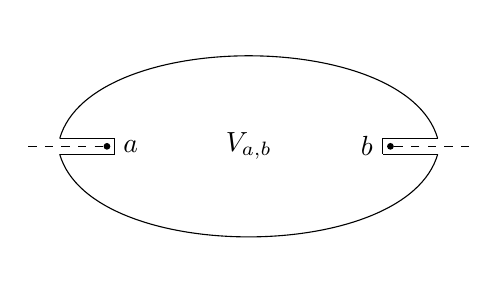
\begin{tikzpicture}

  \draw (-1.5,0) node {$a$};  \draw (1.5,0) node {$b$}; \draw (0,0) node {$V_{a,b}$};
  \filldraw [black] (-1.8,0) circle (1pt); \filldraw [black] (1.8,0) circle (1pt);
    \draw [dashed] (-2.8,0) -- (-1.8,0);   \draw [dashed] (2.8,0) -- (1.8,0);
    \draw (-2.4,0.1) .. controls (-2,1.5) and (2,1.5) .. (2.4,0.1);
    \draw (-2.4,-0.1) .. controls (-2,-1.5) and (2,-1.5) .. (2.4,-0.1);
    \draw (-2.4,-0.1) -- (-1.7,-0.1); \draw (2.4,-0.1) -- (1.7,-0.1);
    \draw (-2.4,0.1) -- (-1.7,0.1); \draw (2.4,0.1) -- (1.7,0.1);
    \draw (-1.7,0.1) -- (-1.7,-0.1); \draw (1.7,0.1) -- (1.7,-0.1);

\end{tikzpicture}

